\documentclass{article}

\usepackage[utf8]{inputenc}
\usepackage[english]{babel}
\usepackage{graphicx}
\usepackage{listings}
\usepackage{xcolor}
\usepackage{float}

\usepackage{rotating}               % 90 degrees image
\usepackage{lscape}                 % landscape 

\usepackage{hyperref}

\usepackage{longtable}
\usepackage{csquotes}               % Use proper \enquote{quotations}

\usepackage[block=ragged,alldates=comp]{biblatex} % Reference management

\usepackage{tikz}
\usepackage{tikz-qtree}

\addbibresource{references.bib}

\usepackage%
[%
left=2cm,% left margin
right=2cm,% right margin
top=3cm, % top margin
bottom=3cm,% bottom margin
a4paper% other options: a0paper, a1paper, a2paper, a3paper, a4paper, a5paper, a6paper, and many more.
]{geometry}

\usepackage{pbox}

\title{DLLGraph}
\author{Youri Klaassens, Nathan Godefroij}
\date{October 2019}

\definecolor{mGreen}{rgb}{0,0.6,0}
\definecolor{mGray}{rgb}{0.5,0.5,0.5}
\definecolor{mPurple}{rgb}{0.58,0,0.82}
\definecolor{backgroundColour}{rgb}{0.95,0.95,0.92}

\setlength{\parindent}{0pt}

\lstdefinestyle{CStyle}{
    backgroundcolor=\color{backgroundColour},   
    commentstyle=\color{mGreen},
    keywordstyle=\color{magenta},
    numberstyle=\tiny\color{mGray},
    stringstyle=\color{mPurple},
    basicstyle=\footnotesize,
    breakatwhitespace=false,         
    breaklines=true,                 
    captionpos=b,                    
    keepspaces=true,                 
    numbers=left,                    
    numbersep=5pt,                  
    showspaces=false,                
    showstringspaces=false,
    showtabs=false,                  
    tabsize=2,
    language=C
}

\tikzset{every tree node/.style={minimum width=2em,draw,circle},
         blank/.style={draw=none},
         edge from parent/.style=
         {draw, edge from parent path={(\tikzparentnode) -- (\tikzchildnode)}},
         level distance=1.5cm}

\lstdefinestyle{ValgrindStyle}{
    backgroundcolor=\color{backgroundColour},   
    breakatwhitespace=false,         
    breaklines=true,                 
    captionpos=b,                    
    keepspaces=true,                 
    numbers=left,                    
    numbersep=5pt,                  
    showspaces=false,                
    showstringspaces=false,
    showtabs=false,                  
    tabsize=2,
    language=C
}

\begin{document}

\begin{titlepage}
	\centering
	\smallbreak                         % smallbreak, medbreak, bigbreak
	\rule{\linewidth}{0.2 mm} \\[0.4 cm]
	{\huge \bfseries Basic Real-Time Operating System}\\
	\smallbreak
	\par{\large targeting the ARMv7-M architecture}      
	\rule{\linewidth}{0.2 mm} \\[1.5 cm]
	\vspace*{0.5 cm}
	\par{\LARGE \textit{ROS01}, Rotterdam \today }\\[1.0 cm]
    
\includegraphics[scale=0.99]{img/HR.png}\\[1.0 cm]	

	


\begin{figure}[!b]
	\begin{minipage}{0.5\textwidth}
		\begin{flushleft} \large
			\emph{Student:}\\
		    Nick van Endhoven\\
            0998831hr.nl\\
            Breda\\
			\end{flushleft}
			\end{minipage}~
			\begin{minipage}{0.5\textwidth}
 
		\begin{flushright} \large
            \emph{Student:}\\
			Youri Klaassens\\
            0996211@hr.nl\\
            Zwaag\\
		\end{flushright}
        
	\end{minipage}\\[2 cm]
\end{figure}
    
    
    
    
	
\end{titlepage}


\tableofcontents
\thispagestyle{empty}

\newpage

\pagenumbering{arabic}
\setcounter{page}{1}

\section{Introduction}

For the Real-time Operating Systems course (ROS01) taught at Rotterdam University of Applied Science,
the authors had to implement a scheduler for a Real-time Operating System developed by one lecturers.
Because these types of programming issues like implementing a scheduler require the programmer to be able to program at a low level and it cannot be assumed that every student following this course is familiar with low level progamming (both in the C programming language and assembler), this course contains multiple assingments to bridge this gap.
The code has been flashed and tested on the CC3220s development board (Figure \ref{fig:cc3220s}). The compiler used is TI v18.12.2.LTS.

What's worth mentioning is that some code snippets in this document make a function call to \texttt{delay\_1sec()}.
Because this is used quite a few times and redundant to have multiple definitions in this document its implementation can be seen in Appendix \ref{subsec:appendix_delay}.


\begin{figure}[H]
    \centering

    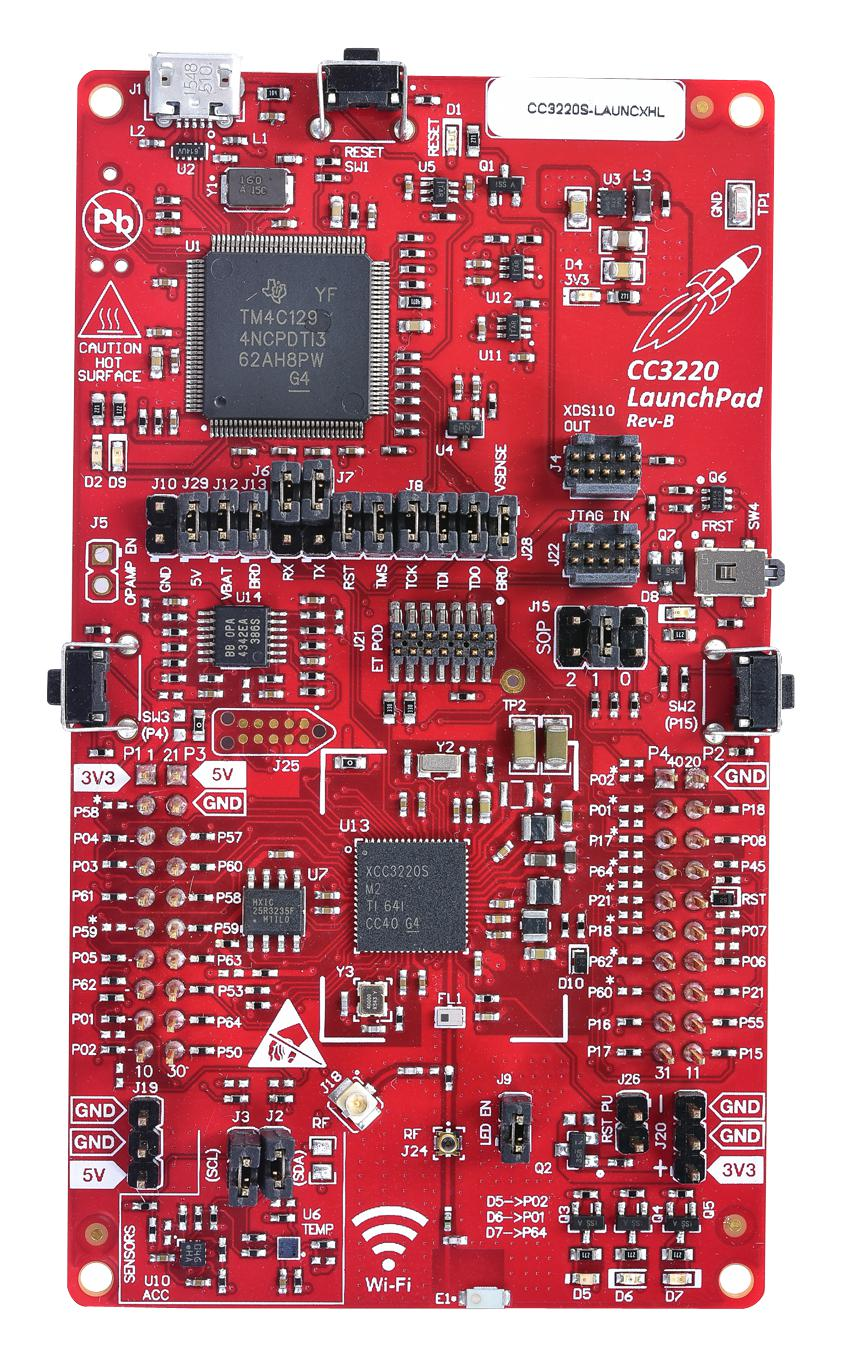
\includegraphics[angle=90,scale=0.2]{img/cc3220s.jpg}

    \caption{The CC3220s development board used during labs}
    \label{fig:cc3220s}

\end{figure}


\end{document}
